\subsubsection{Sensor de nível da água}

  Sensores de nível medem o nível de substâncias que fluem, sejam estes produtos líquidos, pós ou sólidos granulares. Sua medição se dá em detecção de nível, em que existe um sinal que aponta se a substância está acima ou abaixo de um parâmetro, ou medição contínua, onde, dentro de uma faixa de operação, o nível exato é mensurado \cite{quintanilha13}.
  
  A escolha do sensor usado na aplicação depende de vários fatores, entre eles: estado físico do material (alguns sensores são mais adequados para medições de líquidos, enquanto outros têm a melhor aplicação na medição de sólidos granulares ou pós), sensores de temperatura, sendo aplicado em ambientes controláveis. 
  
  Os sensores de níveis que serão implementados nos reservatórios de água do projeto são os sensores do tipo boia magnética da marca Gems Sensores e Controls, eles foram escolhidos por serem confiáveis e baratos, custam em torno de R\$ 120.0, além do mais, sua melhor aplicação é na detecção de nível, pois não tem boa acurácia. Esses sensores também foram escolhidos pela fácil conexão com os microcontroladores e envio de dados. A importância desses sensores no projeto consiste em saber o nível da água para fazer o controle do fluxo da água, decidindo se continua o processo de fluxo ou então se cessa o processo de passagem da água pelo motivo do tanque já estar com sua capacidade máxima atingida. 

  Nesse tipo de sensor, a boia move de acordo com a superfície da água, indicando o nível. A medição pode ser quanto contínua, gerando um sinal analógico ao variar a resistência da haste que segura o flutuador, por exemplo; quanto discreta, simplesmente detectando um limiar, como em uma caixa d’água.
  
%   \begin{figure}[!h]
%     \centering
%     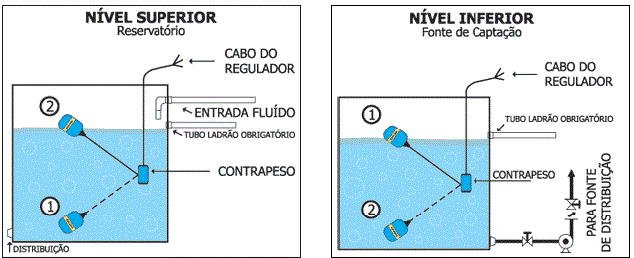
\includegraphics[scale = 0.5]{editaveis/figuras/sensor_nivel_boia}
%     \label{sensor_nivel_boia}
%     \caption{Sensor de nível tipo boia}
%    \end{figure}
%    \FloatBarrier
   
  Sensores do tipo boia magnético funcionam tanto na vertical quanto na horizontal, na horizontal o fechamento do contato ocorre com a aproximação de um campo magnético. Já um flutuador magnético vertical é comumente colocado no topo do tanque e a boia é instalada sob uma mola, que ao ser tencionado, resulta em um movimento vertical tanto do núcleo quanto da haste, levando o magneto para fora, retirando o contato com a chave. 
  
  \begin{figure}[!h]
    \centering
    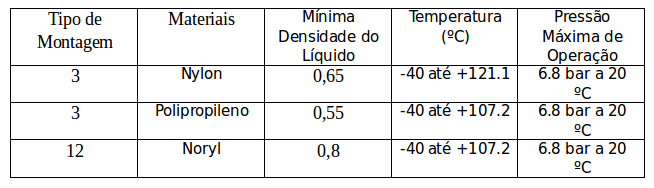
\includegraphics[scale = 0.6]{editaveis/figuras/sensor_nivel_spec}
    \label{sensor_nivel_spec}
    \caption{Especificações do sensor de nível}
   \end{figure}
   \FloatBarrier
   
   \vfill